
\section{Case-Study: Migrating user privileges in web-applications}
\label{sec:casestudy}
To finalize this paper, a use-case for commitments is presented. 

This example describes how a one-time authentication for a web-application can be realized with commitments. 

There are common examples and closed-source libraries which enable developers to implement these features easily, however to keep this paper neutral, only the concept will be shown without going further into detail of several implementations. 

~\newline User-Privileges in web-applications are commonly granted by setting regarding attributes in the session-cookie. As the session-cookie is in the hands of a possibly malevolent user, one of the main-security-measures is to certify the cookie by the server.This behaviour is similiar to the H-MAC (\cite{BeCaKra96} section \textit{the rational} paragraph 3ff ) signing messages in common message exchange applied to cookies. 

As the host usually verifies the cookie in every transaction, he is safe for two main attacks: The user can not create his own cookie, and he cannot alter given cookies. The only way to receive a certified session-cookie is through a successful login.

~\newline Creating a safe login seems like an easy task - but is in itself one of the most important and maintenance-intensive parts of every web-page. Hardening the page, keeping everything up to date and enforce principles such as \textit{Layered Security} (See \cite{Den12} for further reading) requires not only knowledge but time. Therefore simplifying login-procedures, especial for distributed web-applications is a primary goal of web-development. 

~\newline For this cause commitment-schemes can be used to implement a simple \textit{challenge and response} protocol for one time authentication and privilege-migration. For the general setup, see the figure \ref{fig:usecaseone}: 

Alice is the user, Bob-1 is the server which has a functional (and safe) login. Bob-2 is known to Bob-1 and they trust each other. Alice final goal is to be logged in and use Bob-2's services. 
~\newline
~\newline  
The start of this protocol is shown in figure \ref{fig:usecaseone}: In the first step, Alice needs to be logged in and trusted by Bob-1. She then announces her wish to migrate to Bob-2 (e.g. by clicking on a hyperlink) and places a commitment. While these commitments vary from implementation to implementation, they usually contain a mixture of random variables, as well as common connection-attributes such as IP-adress and system-times.   
\begin{figure} [h]
	\centering
	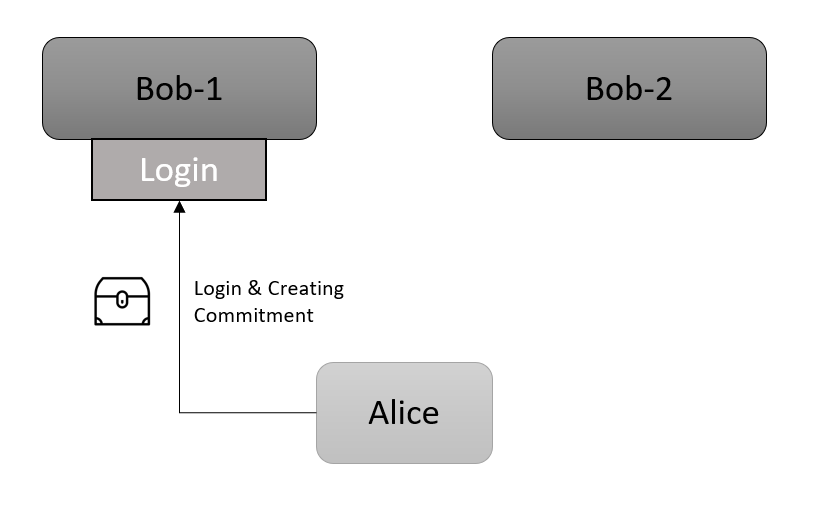
\includegraphics[width=0.6\linewidth]{Images/UseCaseOne}
	\caption[Protocol Start]{Start: Alice log's in, announces her wish to migrate and deposits a commitment}
	\label{fig:usecaseone}
\end{figure}
After the commitment is received by Bob-1, he can start the migration as in figure \ref{fig:usecasetwo}. The first thing to migrate is the commitment itself - with a reference to Alice. This transmission does not need to be encrypted.  

Additionally a secure encrypted message about Alice privileges needs to be exchanged between Bobs. This can either be: 
\begin{enumerate}
	\item The session-cookie itself 
	\item a database reference
	\item a reference to Bob-2's internal security (such as a system-role)
\end{enumerate}
Where most common is the first option, which also enables the possibility for a double-certification, if Bob-2 does not need additional attributes: He therefore signs the full, signed cookie from Bob-1 when granting it again, creating an certification-stack. 

\begin{figure}[h]
	\centering
	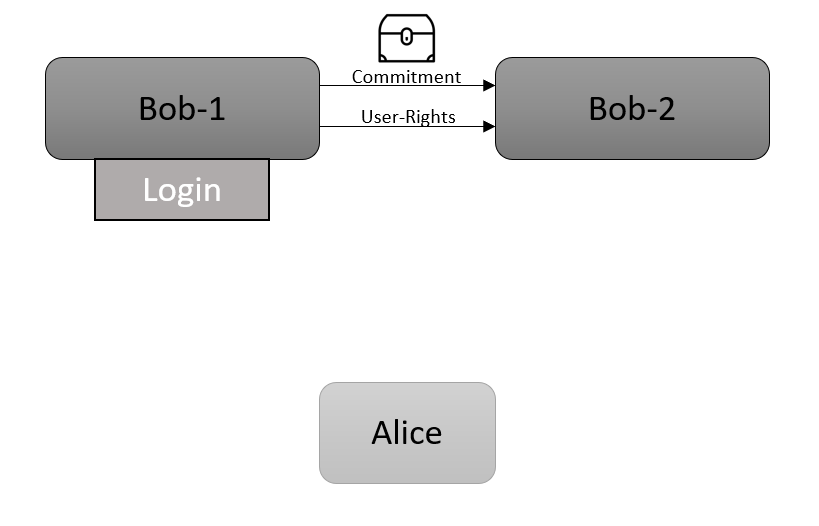
\includegraphics[width=0.6\linewidth]{Images/UseCaseTwo}
	\caption[Protocol Start]{Bob-1 migrates the commitment to Bob-2, as well as additional information for the privileges}
	\label{fig:usecasetwo}
\end{figure}
After Bob-2 successfully received the two messages, he can challenge Alice to reveal the commitment, as shown in figure \ref{fig:usecasethree}. If she is able to, she is granted to privileges regarding the second message. 

She is now able to interact with Bob-2 as if he would have had an usual login.

Most of this protocol can be simply done by user-scripts running in background - it's not required for Alice to enter any random numbers manually. These variables can be migrated with the browser-cache. The Challenge can also be requested and resolved fully automatically, creating the user-experience of a connected web-page.  
\begin{figure}[h]
	\centering
	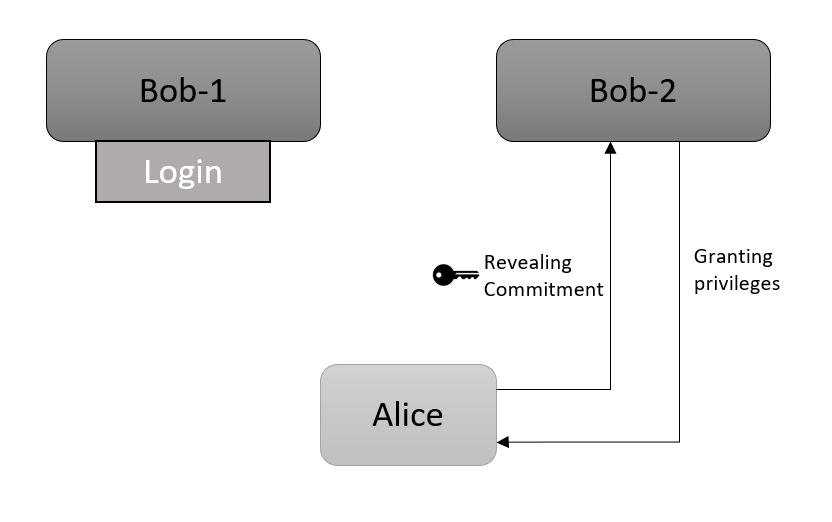
\includegraphics[width=0.6\linewidth]{Images/UseCaseThree}
	\caption[Protocol Start]{Bob-2 challenges Alice to reveal herself, Alice reveals, Bob-2 grants a certified cookie}
	\label{fig:usecasethree}
\end{figure}

~\newline If the communication between parties is secured, and the commitment-scheme has a safe implementation, this one-time authentication is as-safe as the original login. 